\apendice{Especificación de diseño}

\section{Introducción}

La fase de diseño permite planificar un proyecto para su correcta implementación, desarrollo y evolución. En este apartado se van a exponer los diferentes diseños que se han llevado a cabo para obtener unas buenas soluciones a los problemas planteados. Una de las partes más importantes de este proyecto ha sido la investigación, por lo que el diseño en la mayor parte de este proyecto no ha sido necesaria. 
Los diseños realizados han sido:
\begin{enumerate}
    \item \textbf{Diseño de datos}: en esta parte del diseño se mostrarán todas las estructuras de datos utilizadas y una serie de diagramas para entender la estructura del proyecto. 
    \item \textbf{Diseño procedimental}: en esta parte del diseño se mostrará principalmente la comunicación entre el flujo y las implementaciones realizadas.
    \item \textbf{Diseño arquitectónico}: en esta parte del diseño se especificará la arquitectura del proyecto.
\end{enumerate}

En todos los apartados anteriormente mencionados se expondrá, tanto las fases de diseño de la aplicación, como las fases de diseño del proyecto.

\newpage
\section{Diseño de datos}
\textcolor{blue}{Este apartado cuenta con alguna parte del \textit{Diseño de datos} de José Miguel Ramírez Sanz}

\subsection{Diseño de datos del proyecto}
Este proyecto es mayoritariamente un proyecto de investigación por lo que apenas tiene diseño de datos. En este apartado se va a mostrar un diagrama de clases, como se puede observar en la figura \ref{fig:DiagramaClasesProyecto}, con la implementación final de la clase \texttt{PosicionVF} almacenada en el directorio \texttt{src/process}. El diagrama se ha obtenido del proyecto de José Miguel Ramírez Sanz y se le han añadido las nuevas funcionalidades creadas que son las siguientes:
\begin{enumerate}
    \item \texttt{devuelveAngulos()}: esta función devuelve una matriz con todos los ángulos que componen el esqueleto analizado.
    \item \texttt{devuelvePos()}: esta función devuelve una matriz con todos las posiciones relativas al esqueleto y los ángulos calculados. A estos últimos valores se les añadirá una dimensión extra para subsanar los fallos que genera comparar secuencias con distintas dimensiones. 
    \item \texttt{devuelvePosSuperiores()}: esta función devuelve una matriz que contiene las posiciones de la nariz, hombro izquierdo, hombro derecho, cuello, ángulo del cuello izquierdo, ángulo del cuello derecho, codo izquierdo, codo derecho, mano izquierda, mano derecha, ángulo del codo izquierdo, ángulo del codo derecho, ángulo del hombro izquierdo y ángulo del hombro derecho.
    \item \texttt{devuelvePosInferiores()}: esta función devuelve una matriz que contiene las posiciones de la cadera izquierda, cadera derecha, rodilla izquierda, rodilla derecha, ángulo izquierdo de la cadera, ángulo derecho de la cadera, tobillo izquierdo, tobillo derecho, ángulo izquierdo de la rodilla y ángulo derecho de la rodilla. 
\end{enumerate}

Por otro lado, la clase \texttt{Interfaz} es la que se comunica con el flujo de datos (de ahí su nombre), en ella se carga el modelo para posteriormente crean las posiciones.

Además, en el diagrama se pueden observar las relaciones entre las clases más usadas en el código. En este diagrama se puede observar también como se incorpora la herramienta \textit{Detectron2} en el proyecto (clases \emph{cfg, model\_zoo, Instances y DefaultPredictor)}.


Por otra parte, los ficheros generados para localizar y clasificar la secuencia, localizados en \texttt{src/scripts/deploy} son demasiado sencillos como para generar con ellos un diagrama de clases. Esos ficheros cuentan con las siguientes características:
\begin{enumerate}
    \item \texttt{find\_frames.py}: este fichero hay que ejecutarle pasándole como parámetros dos secuencias. La primera de ellas corresponderá a la secuencia de ejercicios concretos y la segunda a la secuencia compuesta por múltiples ejercicios. Una vez recibe las dos secuencias, extrae las posiciones de los archivos con extensión \textit{.pickle} y ejecuta la búsqueda de secuencias. Finalmente informa al usuario de los \textit{frames} de inicio y final de la secuencia. Adicionalmente se han implementado las funciones que clasifican el ejercicio para informar de que tipo es el ejercicio concreto.
    \item \texttt{classify\_exercises.py}: este fichero hay que ejecutarle pasándole como parámetros la secuencia del ejercicio concreto y devolverá una clasificación en función de si se trata de un ejercicio sobre las partes superiores o inferiores del cuerpo humano.
\end{enumerate}

\begin{figure}[H]
    \centering
    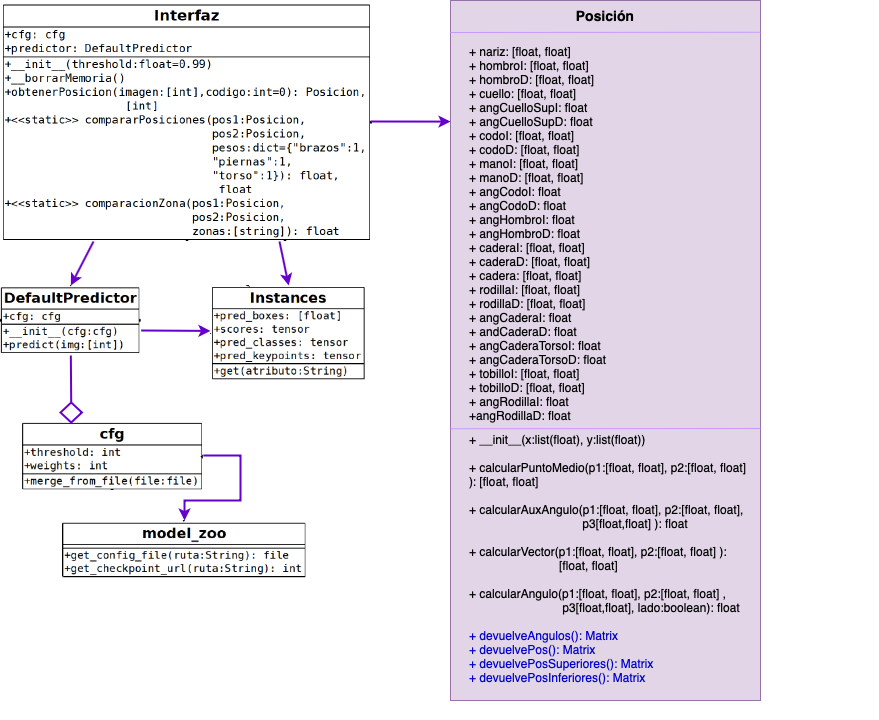
\includegraphics[width=0.9\textwidth]{plantillaLatex-master/img/DiagramaClasesProyecto.png}
    \caption{Diagrama de clases del proyecto.}
    \label{fig:DiagramaClasesProyecto}
\end{figure}

\newpage
\subsection{Diseño de datos de la aplicación}
En este apartado se va a mostrar un diagrama de clases para la aplicación de escritorio, como se puede observar en la figura \ref{fig:DiagramaClasesApp}, en este diagrama se podrán observar las siguientes clases almacenadas en \texttt{app/}:
\begin{enumerate}
    \item \textbf{Window} dentro de \texttt{main.py}, esta clase contiene toda la estructura gráfica de la ventana de la aplicación. En esta clase se pueden apreciar todas las inicializaciones de \textit{frames, labels, botones ...} y las variables que cada uno precisa. Todos estos valores serán almacenados como atributos para poder acceder a ellos con posterioridad desde el resto de clases. 
    \item \textbf{MiddleWindow} dentro de \texttt{MiddleWindow.py}, esta clase tiene como atributo la ventana de inicio. Es la clase encargada de implementar las funciones básicas que debe desarrollar la aplicación, como por ejemplo, mostrar, reproducir o pausar un vídeo, cambiar los colores y habilitar o deshabilitar funcionalidades al cambiar de modo, etc. 
    \item \textbf{PredictWindow} dentro de \texttt{PredictWindow.py}, al igual que la clase anterior, el único atributo que posee es la ventana de inicio. Es la clase encargada de generar el recorte del vídeo, y tiene en cuenta el modo en el que se está trabajando.
\end{enumerate}

\begin{figure}
    \centering
    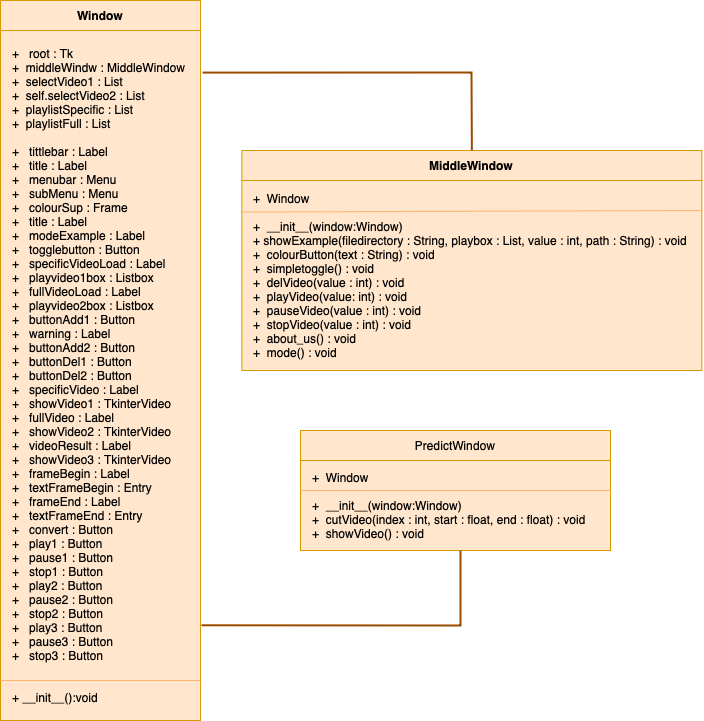
\includegraphics[width=1.1\textwidth]{plantillaLatex-master/img/DiagramaClasesApp.png}
    \caption{Diagrama de clases de la aplicación.}
    \label{fig:DiagramaClasesApp}
\end{figure}

\newpage
\section{Diseño procedimental}
\textcolor{blue}{Este apartado es una ampliación del Diseño de datos de José Luis Garrido Labrador}

\subsection{Diseño procedimental del proyecto}
En este apartado se van a mostrar un par de diagramas de secuencias. En la figura \ref{fig:DiagramaSeqProyecto}, se muestra el proceso general de la aplicación. Este programa contiene una clase \texttt{Ingestor} que se encarga de encolar los \textit{frames} recibidos, y procesarlos. En este proyecto los \textit{frames} vienen procedentes de un único vídeo y lo que programa realiza es ejecutar ese vídeo en bucle por lo que el proceso únicamente acabaría cuando el usuario finaliza el programa. 
\begin{figure}[H]
    \centering
    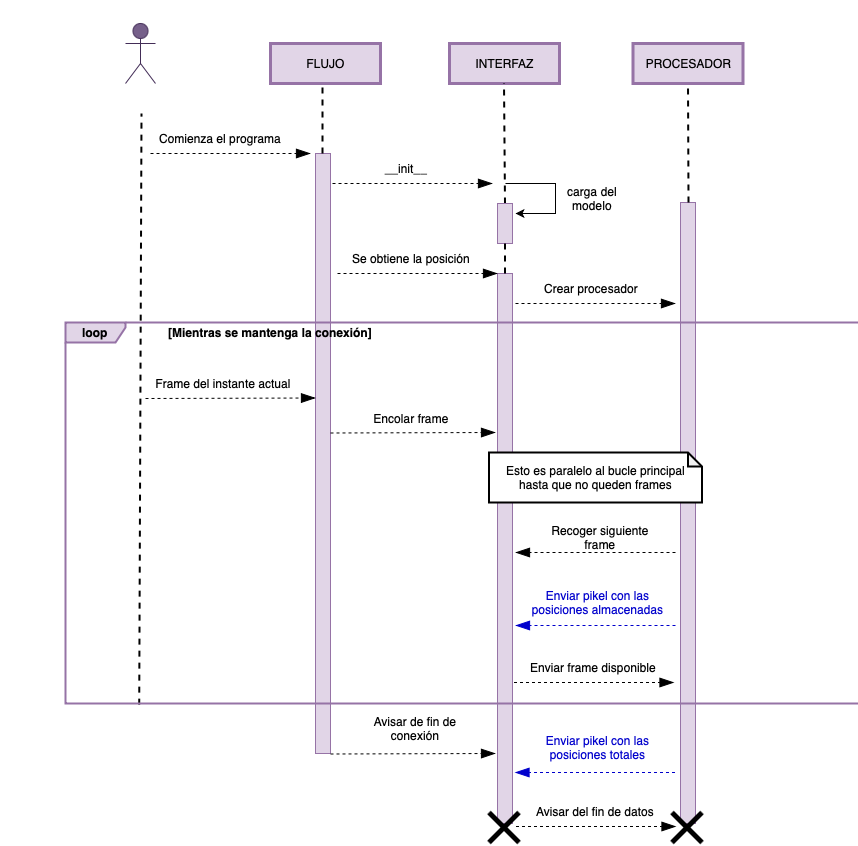
\includegraphics[width=0.9\textwidth]{plantillaLatex-master/img/DiagramaSeqProyecto.png}
    \caption{Diagrama de secuencias de la parte encargada de obtener las posiciones.}
    \label{fig:DiagramaSeqProyecto}
\end{figure}

Por otra parte, en la figura \ref{fig:DiagramaSeqProy2} se puede observar el proceso que se genera para obtener los \textit{frames} de inicio y final y la clasificación del ejercicio. 

\begin{figure}[H]
    \centering
    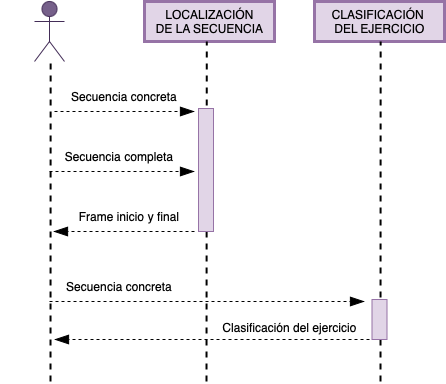
\includegraphics[width=0.7\textwidth]{plantillaLatex-master/img/DiagramaSeqProy2.png}
    \caption{Diagrama de secuencias de la parte encarga de de localizar las secuencias.}
    \label{fig:DiagramaSeqProy2}
\end{figure}


\subsection{Diseño procedimental de la aplicación}
En el diagrama de secuencias que se puede apreciar en la figura \ref{fig:DiagramaSeqApp}, se muestran las tareas principales de la aplicación de escritorio: cargar, reproducir, pausar y detener un vídeo, cambiar el modo de la aplicación y generar un recorte del vídeo que contiene la secuencia de ejercicios completa.

Como se puede apreciar la única diferencia entre el \textit{modo ejemplo ON} y el \textit{modo ejemplo OFF} es que en el segundo hay que especificar los \textit{frames} por los que se desea recortar el vídeo, mientras que en el caso anterior lo hace automáticamente.

\begin{figure}[H]
    \centering
    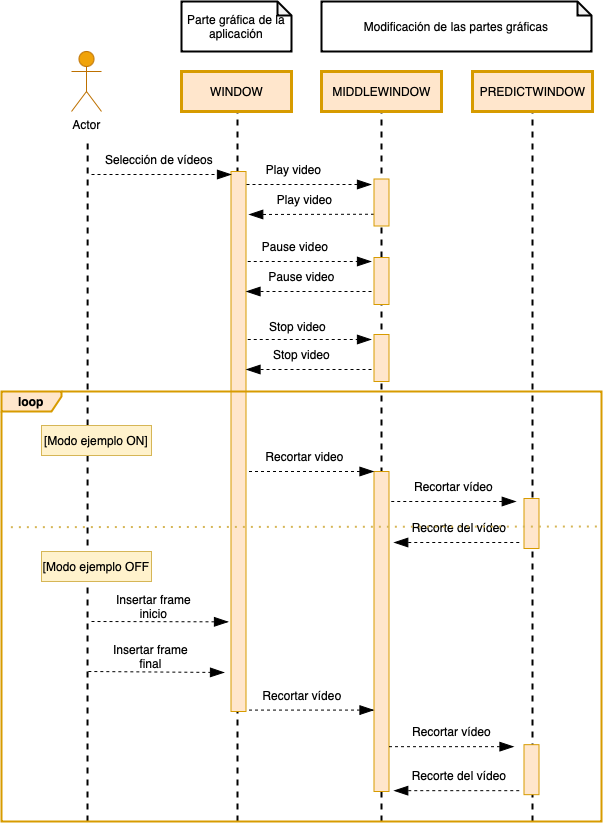
\includegraphics[width=\textwidth]{plantillaLatex-master/img/DiagramaSeqApp.png}
    \caption{Diagrama de secuencias de la aplicación.}
    \label{fig:DiagramaSeqApp}
\end{figure}


\newpage
\section{Diseño arquitectónico}
\textcolor{blue}{Este apartado ha sido extraído del \textit{Diseño de datos arquitectónicos} de José Luis Garrido Labrador}

\subsection{Diseño arquitectónico del proyecto}
Una parte muy esencial de este proyecto es el uso de y despliegue de máquinas virtuales \textit{Docker}. Concretamente hay cuatro tipos de imágenes \textit{Docker}. La primera se
encarga de la serialización de los \textit{frames} y lanzan el \textit{script} de \textit{Python} de
encolado, esta máquina se crea y destruye a voluntad de las conexiones de los pacientes. La segunda y tercera imágenes son el servicio de \textit{Zookeeper} y de \textit{Kafka}. Estas imágenes no se duplican en caso de cambios en las conexiones, únicamente se crean o borran colas. Por último, la cuarta imagen es la transformación del flujo. Se crean o se destruyen según las conexiones de los pacientes y se parametrizan para que consuman un flujo concreto y hagan un procesamiento concreto. El diagrama de despliegue de las máquinas virtuales \textit{docker} se puede observar en la \ref{fig:imgDock}.

\begin{figure}[H]
    \centering
    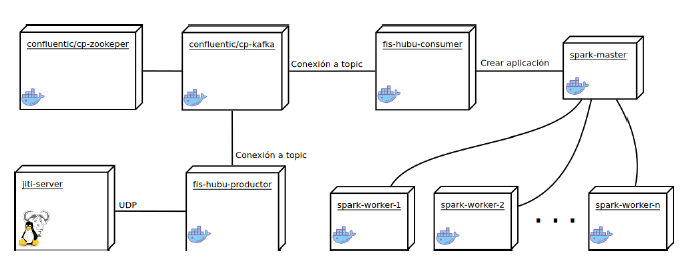
\includegraphics[width=\textwidth]{plantillaLatex-master/img/ImgDocker.png}
    \caption{Diagrama de despliegue de las máquinas virtuales \textit{docker}.}
    \label{fig:imgDock}
\end{figure}

Por otra parte, se ha creado un diagrama con la estructura de los directorios más relevantes del proyecto y se puede observar en la figura \ref{fig:EstructuraDirectoriosSrc}. En esta estructura destacan los directorios:
\begin{enumerate}
    \item \texttt{src/scripts/deploy}: contiene todos los ficheros necesarios para desplegar los servidores e imágenes \textit{Docker}. Además cuenta con los ficheros específicos de este proyecto que localizan y clasifican las secuencias.
    \item \texttt{src/process}: contiene todos los ficheros necesarios para la obtención de las secuencias.
    \item \texttt{src/pruebas}: contiene los distintos \textit{notebooks} generados para explicar las fases del proyecto, a si como muchas de las secuencias generadas y vídeos realizados.
\end{enumerate}

\begin{figure}[H]
    \centering
    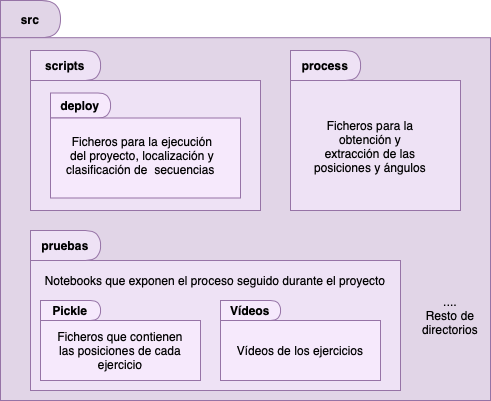
\includegraphics[width=0.55\textwidth]{plantillaLatex-master/img/EstructuraDirectoriosSrc.png}
    \caption{Diagrama de paquetes de la aplicación.}
    \label{fig:EstructuraDirectoriosSrc}
\end{figure}

\subsection{Diseño arquitectónico de la aplicación}
En este apartado se definirá la estructura en paquetes de la aplicación. Como se puede observar en la figura \ref{fig:EstructuraDirectorisApp} la distribución es muy simple. Se almacenan los vídeos en diferentes directorios dentro de la carpeta en la que se encuentran las clases de dicha aplicación. Según el directorio en el que se encuentren cada uno de los vídeos, se cargarán en una sección u otra de la aplicación.

\begin{figure}[H]
    \centering
    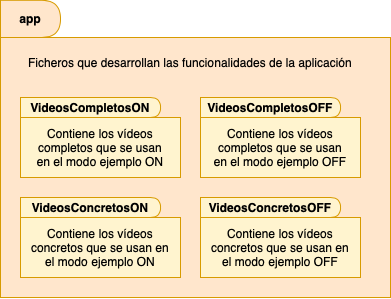
\includegraphics[width=0.55\textwidth]{plantillaLatex-master/img/EstructuraDirectorisApp.png}
    \caption{Diagrama de paquetes de la aplicación.}
    \label{fig:EstructuraDirectorisApp}
\end{figure}
